\documentclass{article}
\usepackage{geometry}
\usepackage{amsmath}
\usepackage{amsfonts}
\usepackage{amssymb}
\usepackage{amsthm}
\usepackage{parskip}
\usepackage{multicol}
\usepackage{xcolor}
\usepackage{fancyhdr}
\usepackage{physics}
\usepackage{graphicx} % Required for inserting images
\usepackage{hyperref}
\usepackage{enumitem}
\usepackage{mathtools}

% commands
\newcommand{\deq}{\vcentcolon=}
\newcommand{\idd}{\text{đ}}
\newcommand{\nimplies}{\centernot\implies}
\newcommand{\vc}[1]{\boldsymbol{#1}}

% margin settings
\geometry{
    a4paper,
    left=7mm,
    right=7mm,
    top=2cm,
    bottom=7mm
}

% testing
\usepackage{blindtext}

% proof environments
\newtheorem{definition}{Definition}[section]
\newtheorem{theorem}{Theorem}[section]
\newtheorem{corollary}{Corollary}[theorem]
\newtheorem{lemma}[theorem]{Lemma}
\newtheorem*{remark}{Remark} % unnumbered remarks

% header and footer
\pagestyle{fancy}
\fancyfoot{} % removes footer
\fancyhf{}
\renewcommand{\headrulewidth}{0.5pt}
\fancyhead[L]{Honours complex variables}
\fancyhead[R]{\thepage}

\begin{document}

\begin{multicols*}{3}
% starred environment ensures text remains in same column
\noindent

\subsubsection*{D1.1.1: Complex numbers}
Let $z=x+iy$ and $w=a+ib$ where $x,y,a,b\in\mathbb{R}$.
Then $z$ and $w$ are complex numbers. Furthermore:
\begin{enumerate}
    \item $z=w$ \textbf{if{}f} $x=a$ and $y=b$.
    
    \item $\Re(z)\deq x$ and $\Im(z)\deq y$.
    
    \item $|z|\deq\sqrt{x^2+y^2}$
    
    \item The \textbf{complex conjugate} of $z$ is:
    $$\overline{z}\deq x-iy.$$

    \item Addition and multiplication:
    $$(x+iy)+(a+ib)=(x+a)+i(y+b)$$
    $$(x+iy)(a+ib)=(xa-yb)+i(xb+ya).$$

    \item $\mathbb{C}\deq\{x+iy:x,y\in\mathbb{R}\}$
\end{enumerate}
with rule $i^2=-1$.

\subsubsection*{L1.1.3}
Let $u,w,z\in\mathbb{C}$ where $z=x+iy$. Then:
\begin{enumerate}
    \item $z+w=w+z$ and $zw=wz$.
    
    \item $u+(z+w)=(u+z)+w$
    
    \item $u(zw)=(uz)w$
    
    \item $u(z+w)=uz+uw$
    
    \item $z+0=z$ and $1z=z$.
    
    \item $\exists\bigl(-z\deq-x+i(-y)\bigr)$:
    $z+(-z)=0$.

    \item $\exists z^{-1}: zz^{-1}=1$ where:
    $$z^{-1}\deq\frac{x}{x^2+y^2}+i\frac{-y}{x^2+y^2}.$$
\end{enumerate}

\subsubsection*{D1.1.5 and D1.1.7: Polar form}
Let $z\in\mathbb{C}$ and $z=x+iy$. Then:
\begin{align*}
    z
    &=r(\cos\theta+i\sin\theta) \\
    &=re^{i\theta}
\end{align*}
for $r=\sqrt{x^2+y^2}$ in complex plane.
\begin{center}
    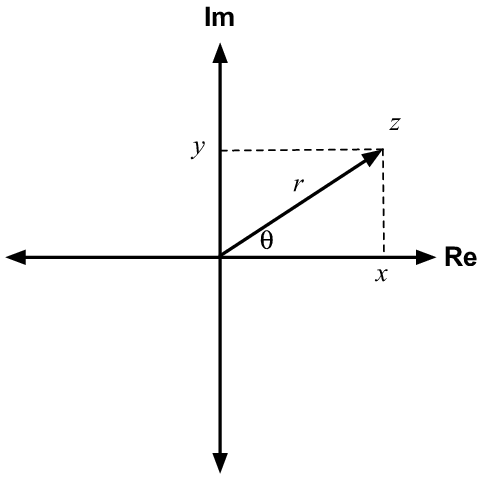
\includegraphics[scale=0.2]{f0.png}
\end{center}

\subsubsection*{L1.1.6}
Let $\theta,\phi\in\mathbb{R}$ and $n\in\mathbb{Z}$. Then:
\begin{enumerate}
    \item $e^{i(\theta+\phi)}=e^{i\theta}e^{i\phi}$
    
    \item $e^{in\theta}=(e^{i\theta})^n$
\end{enumerate}
due to de Moivre's formula:
$$\cos n\theta+i\sin n\theta=(\cos \theta+i\sin \theta)^n.$$

\newcolumn

\subsubsection*{L1.1.9}
Let $z,w\in\mathbb{C}$. Then:
\begin{enumerate}
    \item $|z|=0$ \textbf{if{}f} $z=0$.
    
    \item $|\overline{z}|=|z|$
    
    \item $|zw|=|z||w|$
    
    \item $\overline{\overline{z}}=z$
    
    \item $|z|^2=z\overline{z}$
    
    \item $\overline{z+w}=\overline{z}+\overline{w}$
    
    \item $\overline{zw}=\overline{z}\hspace{0.02in}\overline{w}$
    
    \item $|\Re(z)|\leq|z|$ and $|\Im(z)|\leq|z|$.
    
    \item $\Re(z)=\frac{1}{2}(z+\overline{z})$
    
    \item $\Im(z)=\frac{1}{2i}(z-\overline{z})$.
\end{enumerate}

\subsubsection*{L1.1.10 -- 11: Triangle inequalities}
Let $z,w\in\mathbb{C}$. Then:
\begin{enumerate}
    \item $|z+w|\leq|z|+|w|$
    
    \item $||z|-|w||\leq|z-w|$.
\end{enumerate}

\subsubsection*{D1.1.12: Argument of $z$}
Let $z=|z|e^{i\theta}$. Then:
$$\arg(z)\deq\theta\in(-\pi,\pi]$$
with period $2\pi$.

\subsubsection*{P1.1.14}
Let $z,w\in\mathbb{C}$. Then:
\begin{enumerate}
    \item $\arg(zw)=\arg(z)+\arg(w)$
    
    \item $\arg(\overline{z})=-\arg(z)$
\end{enumerate}
and holds under modulo $2\pi$.

\subsubsection*{D1.2.1: Open and closed $\epsilon$-discs}
Let $z_0\in\mathbb{C}$ and $\epsilon>0$.
\begin{enumerate}
    \item An \textbf{open} $\epsilon$-disc
    centred at $z_0$ is:
    $$D_{\epsilon}(z_0)
    \deq\{z\in\mathbb{C}:|z-z_0|<\epsilon\}.$$

    \item A \textbf{closed} $\epsilon$-disc
    centred at $z_0$ is:
    $$\overline{D}_{\epsilon}(z_0)
    \deq\{z\in\mathbb{C}:|z-z_0|\leq\epsilon\}.$$
\end{enumerate}
A \textbf{punctured} $\epsilon$-disc centred at $z_0$ is:
$$D'_{\epsilon}(z_0)\deq\{z\in\mathbb{C}:0<|z-z_0|<\epsilon\}.$$

\subsubsection*{D1.2.2: Open sets}
Let $U\subset\mathbb{C}$. Set $U$ is \textbf{open} if:
$$\forall z_0\in U;\exists\epsilon>0:D_{\epsilon}(z_0)\subseteq U.$$
Subset $F$ is \textbf{closed} if
$\mathbb{C}\hspace{0.02in}\backslash\hspace{0.02in} F$ is open.

A \textbf{neighbourhood} of point $z_0\in\mathbb{C}$
is an open set that contains $z_0$.

\subsubsection*{L1.2.3}
Punctured disc $D'_{\epsilon}(z_0)$ is open.

\subsubsection*{D1.2.4: Limit points}
Let $S\subseteq\mathbb{C}$. $z_0$ is a \textbf{limit point} of $S$ if:
$$\forall\epsilon>0; D'_{\epsilon}(z_0)\cap S\neq\emptyset.$$
The \textbf{closure} of $S$ is set $\overline{S}$ and contains $S$
and \textbf{all} its limit points.

\subsubsection*{L1.2.6}
Let $S\subseteq\mathbb{C}$.
$S$ is closed \textbf{if{}f} $S=\overline{S}$.

\subsubsection*{D1.2.7: Bounded sets}
Let $S\subseteq\mathbb{C}$. Set $S$ is \textbf{bounded} if:
$$\forall z\in S;\exists M>0:|z|\leq S.$$

\subsubsection*{D1.2.8: $\epsilon$-N convergence}
Let $\mathbb{N}=\{0,1,2,\dots\}$.

Let $(z_n)_{n\in\mathbb{N}}\subseteq\mathbb{C}$ be a sequence
and $z\in\mathbb{C}$.
Then $\displaystyle\lim_{n\rightarrow\infty}z_n=z$ if:
\begin{align*}
    &\forall\epsilon>0;\exists N\in\mathbb{N}:\forall n\geq N \\
    &\implies |z_n-z|<\epsilon.
\end{align*}

\subsubsection*{L1.2.9}
Let $z_n,z\in\mathbb{C}$ where $z_n=a_n+i b_n$.

Then $\displaystyle\lim_{n\rightarrow\infty}z_n=z$ \textbf{if{}f}:
$$\Re(z)=\lim_{n\rightarrow\infty}a_n
\hspace{0.05in}\text{and}\hspace{0.05in}
\Im(z)=\lim_{n\rightarrow\infty}b_n.$$

\subsubsection*{L1.2.10}
Let $S\subseteq\mathbb{C}$ and $z\in\mathbb{C}$.
Then $z\in\overline{S}$ \textbf{if{}f}:
$$\exists z_n\in S: z=\lim_{n\rightarrow\infty}z_n.$$

\subsubsection*{D1.2.11: Cauchy sequences}
$z_n$ is a Cauchy sequence if:
\begin{align*}
    &\forall\epsilon>0;\exists N\in\mathbb{N}:
    \forall n,m\geq N \\
    &\implies |z_n-z_m|<\epsilon.
\end{align*}

\subsubsection*{L1.2.12}
$z_n$ is convergent \textbf{if{}f} $z_n$ is Cauchy.

\subsubsection*{D1.2.14: Bounded sequences}
$z_n$ is bounded if:
$$\forall n\in\mathbb{N};\exists M>0:|z_n|\leq M.$$

\subsubsection*{L1.2.15: Bolzano-Weierstrass}
Let $z_n$ be a bounded sequence. Then:
$$\exists (z_{n_k})_{k,n_k\in\mathbb{N}}:
\lim_{k\rightarrow\infty}z_{n_k}=z\in\mathbb{C}$$
or that $z_n$ has a convergent subsequence.

A selection of a sequence is a subsequence.

\newcolumn

\subsubsection*{Remark}
define a complex valued function

\subsubsection*{D1.3.1: Bounded functions}

\subsubsection*{D1.3.2: $\epsilon$-$\delta$ convergence}

\subsubsection*{L1.3.3 ?}

\subsubsection*{L1.3.4}
results on function limits

\subsubsection*{L1.3.5}
limit algebra

\subsubsection*{D1.3.6: $\epsilon$-$\delta$ continuity}

\subsubsection*{L1.3.7}

\subsubsection*{L1.3.8}
composition of functions are also continuous

\subsubsection*{L1.3.9}

\subsubsection*{L1.3.10}

\newpage

\end{multicols*}

\end{document}